%%__________________________________________________________________||
\section{Introduction}
\label{sec:introduction}

Supersymmetry (SUSY)~\cite{ref:SUSY-1, ref:SUSY0, ref:SUSY1,
  ref:SUSY2, ref:SUSY3, ref:SUSY4, ref:hierarchy1, ref:hierarchy2}
provides a complete, renormalisable extension to the Standard Model
(SM) that can provide a solution to the hierarchy problem of the SM
Higgs boson~\cite{ref:atlashiggsdiscovery, ref:cmshiggsdiscovery}
providing SUSY is realised at the TeV scale. Further, the assumption
of R-parity conservation~\cite{Farrar:1978xj} has important
consequences for collider phenomenology and cosmology. Supersymmetric
particles (sparticles) such as gluinos and squarks are expected to be
produced in pairs at the LHC and promptly decay to SM particles and
the lightest stable supersymmetric particle (LSP), which is generally
assumed to be a weakly interacting, massive neutralino and a dark
matter candidate. The characteristic signature of SUSY production at
the LHC is a final state of multijets accompanied by significant
missing transverse momentum, \ptvecmiss.

The new energy frontier of the LHC during Run~2 provides a unique
opportunity to search for the characteristic signatures of TeV-scale
sparticles~\cite{atlas-12, atlas-13, cms-12, cms-13}. This Physics
Analysis Summary presents an inclusive search for the pair production
of massive coloured sparticles in hadronic final states with one or
more energetic jets and missing transverse momentum, performed in pp
collisions at a centre-of-mass energy $\sqrt{s} = 13\TeV$. The
analysed data sample corresponds to an integrated luminosity of $2.6
\pm 0.1 \fbinv$~\cite{lumi} collected by the Compact Muon Solenoid
(CMS) experiment. A detailed description of the CMS detector can be
found in Ref.~\cite{ref:CMS}. Previous iterations of this search have
been performed in pp collisions at $\sqrt{s} = 7$~\cite{RA1Paper,
  RA1Paper2011, RA1Paper2011FULL}, $8$~\cite{RA1Paper2012, RA1Parked},
and $13\TeV$~\cite{RA1Paper2015}.

The search strategy is based around two key aspects in order to
achieve a robust, inclusive search capable of exploiting the potential
of the new LHC energy frontier under the challenging conditions of new
beam and detector configurations early in Run~2. First, multiple tight
selection criteria are employed to suppress multijet production, a
manifestation of quantum chromodynamics (QCD), to a negligible level
relative to all other SM background processes. Second, the
experimental acceptance to a potential signal is maximised through the
use of trigger conditions that maintain the same low thresholds
employed during Run~1.

The strategy is built around the use of the kinematic variable
\alphat~\cite{Randall:2008rw, RA1Paper}, which provides powerful
discrimination against multijet production. The \alphat variable is
constructed from jet-based quantities to provide robust discriminating
power between sources of genuine and misreconstructed missing
transverse momentum, making it suitable for early searches operating
at new energy and luminosity frontiers. The \alphat variable is
utilised as part of the trigger conditions, providing high performance
in terms of maintaining low thresholds for a given trigger
bandwidth. Further variables are also employed to discriminate against
multijet production and suppress this background process to a
negligible level. The $\Delta\phi^{*}_{\rm min}$~\cite{RA1Paper}
variable exploits azimuthal angular information and also provides
strong rejection power against multijet events, including rare
energetic events in which neutrinos carry a significant fraction of a
jet's energy due to semileptonic decays of heavy-flavour mesons.

%The search is devised around the kinematic variable
%\alphat~\cite{Randall:2008rw, RA1Paper} that provides powerful
%discrimination against multijet production, a manifestation of quantum
%chromodynamics (QCD), and adheres to an inclusive strategy with the
%aim of providing sensitivity to the widest possible range of SUSY
%models. The \alphat variable is constructed from jet-based quantities
%to provide robust discriminating power between sources of genuine and
%misreconstructed missing transverse momentum, making it suitable for early
%searches. A further variable that exploits azimuthal angular
%information, known as $\Delta\phi^{*}_{\rm min}$~\cite{RA1Paper}, is
%also employed to suppress QCD multijet production, including potential
%contributions from semileptonic heavy-flavour decays, to a negligible
%level.

The search is based on an examination of the number of reconstructed
jets per event, the number of these jets identified as originating
from bottom quarks, and the scalar and vector sums of transverse
momenta of these jets. 
%The search exploits the use of \mht templates derived from simulation,
%which are extensively validated in data control regions. 
These discriminating variables provide sensitivity to the different
production mechanisms of massive coloured sparticles at hadron
colliders (\ie squark-squark, squark-gluino, and gluino-gluino),
third-generation squark signatures, and a large range of mass
splittings between the parent sparticle and the LSP,
respectively. Interpretations of the result %are
\fixme{\it will be} provided in the parameter space of simplified
models~\cite{Alwall:2008ag, Alwall:2008va, sms} that represent the
pair production of gluinos and their subsequent prompt decays.
%to four quarks and two LSPs via off-shell squarks of light or heavy
%flavour, as illustrated in Fig.~\ref{fig:feyn}.

%\begin{figure*}[thb]
%\centering
%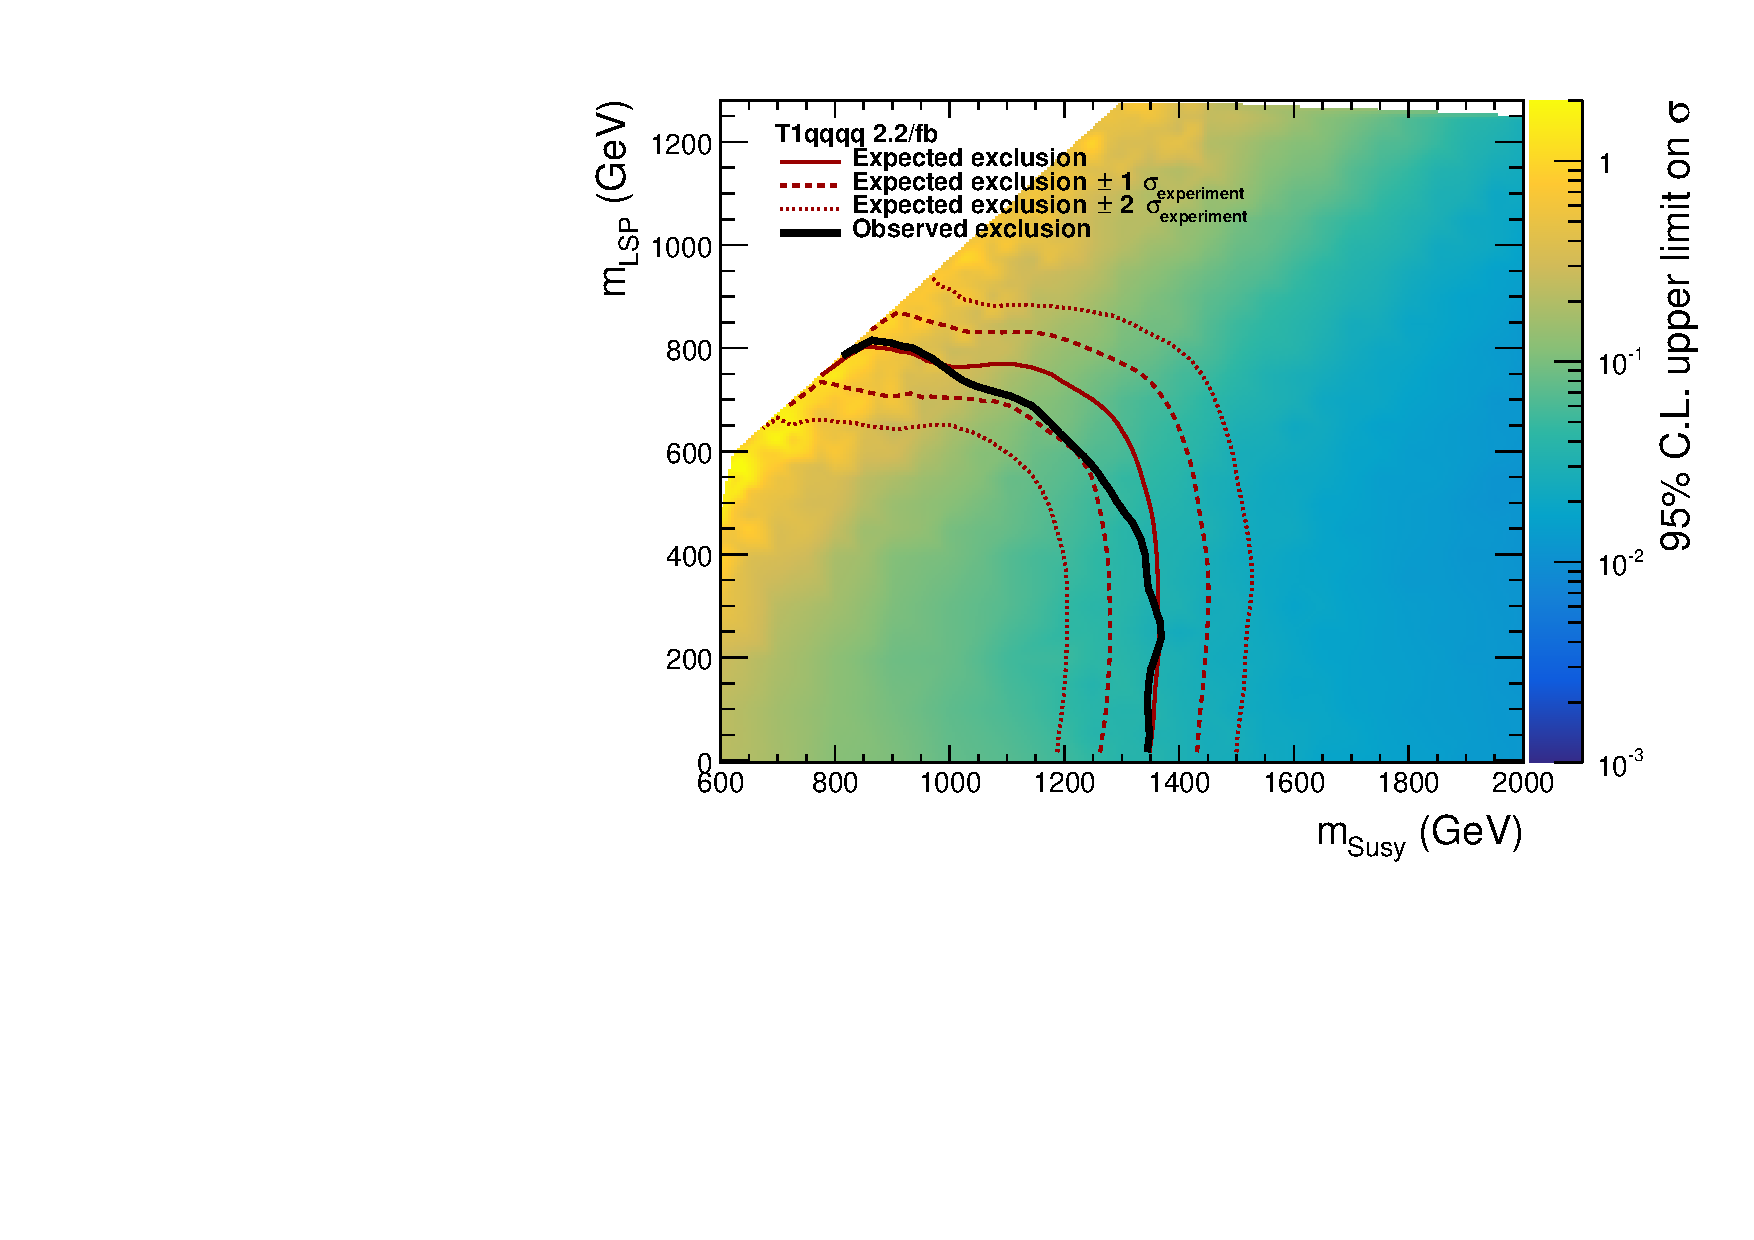
\includegraphics[width=0.45\linewidth]{T1qqqq.pdf} \,
%%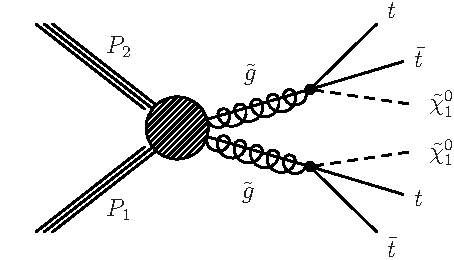
\includegraphics[width=0.32\linewidth]{T1tttt.pdf}
%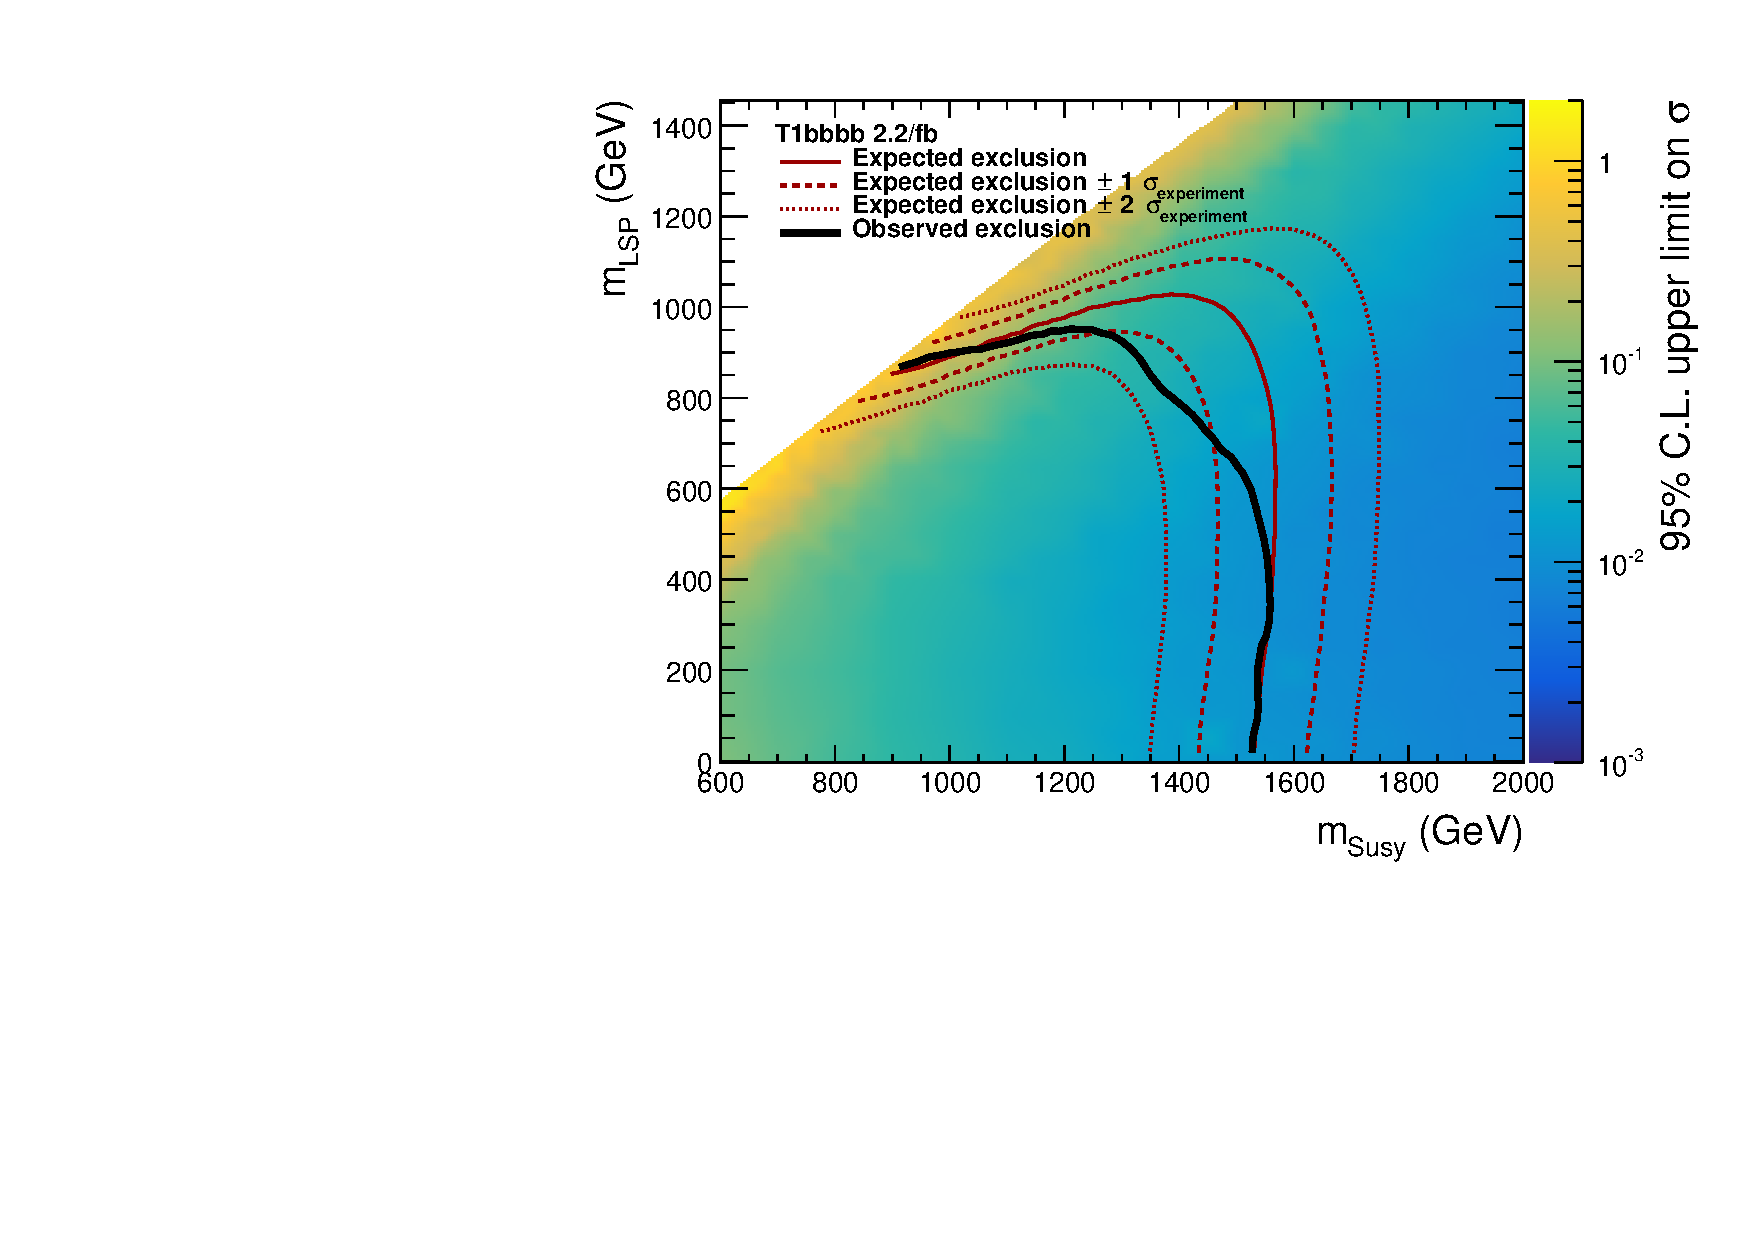
\includegraphics[width=0.45\linewidth]{T1bbbb.pdf}
%\caption{Representations of simplified models comprising the pair
%  production of gluinos and prompt three-body decays to
%  $q\bar{q}\chiz_{1}$ (left) and $b\bar{b}\chiz_{1}$ (right) via an
%  off-shell light-flavour or bottom squark, respectively.}
%\label{fig:feyn}
%\end{figure*}


%%__________________________________________________________________||
